\documentclass{article}

\usepackage[paper=letterpaper,margin=2.5cm]{geometry} % Set Margins

%% Math and math fonts
\usepackage{amsmath, amsthm, amssymb, amsfonts}
\usepackage{bbm} % for \mathbbm{1}

% date
\usepackage[nodayofweek]{datetime}

% Color
\usepackage{color, xcolor}

% Misc
\usepackage{environ}  % \collect@body in asmmath
\usepackage{graphicx} % \includegraphics options
\usepackage{mdframed} % text boxes
\usepackage{indentfirst} % Indent first paragraph after section header
\usepackage[shortlabels]{enumitem} % Control enumerate items with [(a)]
\usepackage{comment} % Comments
\usepackage{fancyhdr} % Headers and footers

% Tables
\usepackage{array}

% Sub-figures and figure placement
\usepackage{caption}
\usepackage{subcaption}
\usepackage{float} 

% Graphing
\usepackage{pgfplots}
\pgfplotsset{compat=1.17}
\usepackage{tikz}

% Title Placement
\usepackage{titling}
\setlength{\droptitle}{-6em}

%set indent to 
\setlength{\parindent}{0pt}

% Hyper refs
\usepackage{hyperref}
\hypersetup{
    colorlinks=true,
    linkcolor=blue,
    urlcolor  = blue,
    filecolor=magenta,      
    urlcolor=blue,
    citecolor = blue,
    anchorcolor = blue
}

% % Citation management
\usepackage{natbib}
\bibliographystyle{abbrvnat}
\setcitestyle{authordate,open={(},close={)}}

\pagestyle{fancy}

\usepackage[paper=letterpaper,margin=2.5cm]{geometry} % Set Margins

%% Math and math fonts
\usepackage{amsmath, amsthm, amssymb, amsfonts}
\usepackage{bbm} % for \mathbbm{1}

% date
\usepackage[nodayofweek]{datetime}

% Color
\usepackage{color, xcolor}

% Misc
\usepackage{environ}  % \collect@body in asmmath
\usepackage{graphicx} % \includegraphics options
\usepackage{mdframed} % text boxes
\usepackage{indentfirst} % Indent first paragraph after section header
\usepackage[shortlabels]{enumitem} % Control enumerate items with [(a)]
\usepackage{comment} % Comments
\usepackage{fancyhdr} % Headers and footers

% Tables
\usepackage{array}

% Sub-figures and figure placement
\usepackage{caption}
\usepackage{subcaption}
\usepackage{float} 

% Graphing
\usepackage{pgfplots}
\pgfplotsset{compat=1.17}
\usepackage{tikz}

% Title Placement
\usepackage{titling}
\setlength{\droptitle}{-6em}

%set indent to 
\setlength{\parindent}{0pt}

% Hyper refs
\usepackage{hyperref}
\hypersetup{
    colorlinks=true,
    linkcolor=blue,
    urlcolor  = blue,
    filecolor=magenta,      
    urlcolor=blue,
    citecolor = blue,
    anchorcolor = blue
}

% % Citation management
\usepackage{natbib}
\bibliographystyle{abbrvnat}
\setcitestyle{authordate,open={(},close={)}}

% ----------------------------------------
% TITLE
% ----------------------------------------

\pagestyle{fancy}

\lhead{Creel}
\chead{Week Four}
\rhead{AMES}

\title{AMES Section Notes -- Week Four}
\author{Andie Creel}

\begin{document}
\maketitle

\section{Quasi concavity/convexity}

Consider the function 
\begin{align*}
    F(x_1, x_2) = x_1^{1/2} x_2^{1/2}
\end{align*}
$F(x_1, x_2)$ maps from $R^2$ to $R^1$, 
\begin{align*}
    R^2 \to R^1.
\end{align*}

To visualize $F(x_1, x_2)$ we need to do it in $R^3$ (3-D) because we need a dimension for both inputs and the output.\\

To visualize a $n$ dimensional function you need a $n+1$ dimensions because you need an additional dimension for the output.

\begin{figure}[htp]
    \centering
        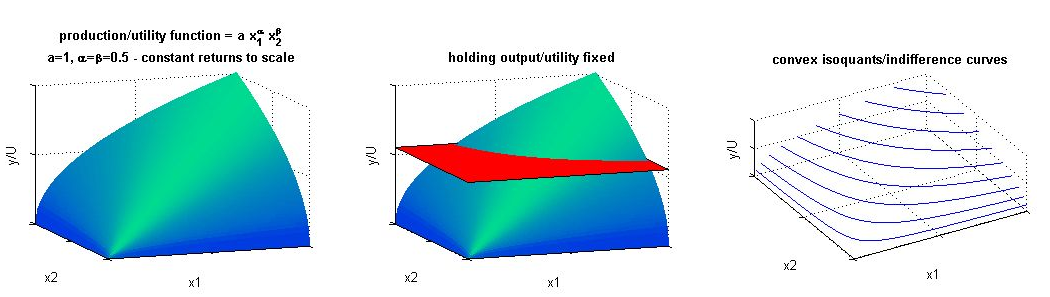
\includegraphics[width=1\textwidth]{Screen Shot 2023-09-18 at 2.03.06 PM.png}
    % \caption{convex and concave }
    % \label{fig:sample}
\end{figure}

Source: \url{https://www2.hawaii.edu/~fuleky/anatomy/anatomy.html}\\



If a function is in $R^2$ (\textit{i.e.} it takes two inputs) then you must evaluate if  the function is convex or concave in $R^3$. That will determine if the function is convex or concave. But then if you graph you function in $R^2$ space (meaning you're not using an additional dimension for the output) the function may look convex or concave in the lower dimension. Despite how it looks in the lower dimension, you must determine if it's quasi-convex or quasi-concave from the higher dimension.  \\

If the function is convex in $R^3$ (\textit{e.g.} it looks like a bowl), when you graph it in $R^2$ it's quasi-convex. If the function is concave in $R^3$ (\textit{e.g.,} it looks like a hat), when graphed in $R^2$ it's quasi-concave. \\

\textit{Verbally explain what would happen if you set $ F(x_1, x_2)$ to a constant $C$ and solve for $ x_1 = g(x_2, C)$. Is $g(\cdot)$ convex or concave?}


\section{Log rules:}
Consider the equation 
\begin{align*}
    y = \alpha x e^{\beta x}\nu
\end{align*}

where $y$ is an endogenous-variable (determined by the system \textit{aka} dependent variable), $x$ is a variable (aka independent variable), $\alpha$ is an exogenous parameter, $\beta$ is an exogenous parameter, and $\nu$ is measurement error.\\

You want to use log rules so that you can get this to look like an equation where you could use linear regression to estimate $\alpha$ and $\beta$. That mean we want an endogenous variable that's a function of a constant, a linear term with the dependent variable, and an error term.

\begin{align*}
    \log(y) &= \log(\alpha x e^{\beta x}\nu) \\
    \log(y) &= \log(\alpha) + \log(x) + \log(e^{\beta x}) +\log(\nu)\\
    \log(y) &= \log(\alpha) + \log(x) + \beta x \log(e) + \log(\nu)\\
    \log(y) &= \log(\alpha) + \log(x) + \beta x + \log(\nu)\\
    \log(y) - \log(x) &= \log(\alpha) + \beta x + \log(\nu) \\
    \log(y/x) &= \log(\alpha) + \beta x + \log(\nu)
\end{align*}



\end{document}